%
% string matching writeup...
%

\documentclass{llncs}
\pagestyle{empty}
\usepackage{makeidx}  % allows for indexgeneration
%
\usepackage[dvips]{graphicx}    % needed for including graphics e.g. EPS, PS
\usepackage{epsfig}
\usepackage{url}
\usepackage{pseudocode}
\usepackage{comment}
\usepackage{authblk}
\usepackage{color}
\usepackage{newalg}
\usepackage{subfigure}

\begin{document}
\renewcommand{\labelenumi}{(\Alph{enumi})}
\renewcommand{\labelenumii}{(\alph{enumii})}

\frontmatter          % for the preliminaries
%
\pagestyle{headings}  % switches on printing of running heads

\mainmatter              % start of the contributions
%
\title{Bridging the gap: improving local multiple alignment with gapped extension.}
%
\titlerunning{procrastination for local multiple alignment}  % abbreviated title (for running head)
%                                     also used for the TOC unless
%                                     \toctitle is used
\author{Todd,Aaron,MarkRagan,Xavier,anybodyelse?}

%\institute{
%Algorithms and Genetics Group, Dept. of Computer Science, Technical Univ. of Catalonia, Barcelona, Spain\\
%\email{treangen@lsi.upc.edu},\\
%}
%
\authorrunning{<Quijote> et al.}   % abbreviated author list (for running head)

\maketitle


\begin{abstract}
The identification of homologous DNA via sequence alignment is a basic building block in comparative genomics.  We present a method for accurately and sensitively identifying homologous DNA sequence in multiple genomes. Our method is based around an efficient heuristic for local multiple alignment, featuring a novel method for gapped extensions. In practice, we are able to sensitively identify conserved, potentially repetitive, regions in one or more DNA sequences.  The GPL implementation of our algorithm in C++ is
called \texttt{procrastAligner} and is freely available from
\url{http://gel.ahabs.wisc.edu/procrastination}
\end{abstract}




\section{ Introduction }

The importance of accurate homology identification to comparative genomics can not be overestimated (cite Kumar 2006/7 GenomeResearch paper). To date, pairwise local sequence alignment methods~\cite{blast,ssearch...} have been the prevailing technique to identify homologous nucleotides.  When more than two copies of a homologous sequence element are present in the data, pairwise homology detection methods generate a listing of all possible pairs of homologous elements.  Apart from the obvious inefficiency of considering all pairwise homology relationships, a collection of pairwise alignments is not ideal because they are rarely amenable to comparative genomic and phylogenetic analysis without further processing into a multiple alignment.

Local pairwise alignments can be merged to create a multiple alignment by a variety of methods~\cite{multiz,repeatgluer,aba,dialign...}. Such methods commonly assume that pairwise homology relationships are transitive, such that if nucleotide $a$ is homologous to nucleotide $b$, and $b$ is to $c$, then $a$ must also be homologous to $c$.  Thus, in order to merge pairwise alignments, such methods must tackle the challenging problem of resolving inconsistent transitive homology relationships.  Pairwise alignment has been demonstrated to be less accurate than multiple alignment, especially when dealing with a large number of divergent sequences~\cite{MLAGANpaper,AuberGene,others?,...}.  As the number of homologous sequences grows, we might expect that the number of inconsistent relationships in a collection of pairwise alignments would grow quadratically, whereas a direct multiple alignment method would provide an increasingly accurate alignment.  Highly repetitive regions in the input sequences can cause particularly nasty efficiency problems for pairwise methods, as they must conduct $O(n^{2})$ pairwise comparisons for each of the repeated regions.  Mammalian Alu repeats and IS elements in microbes are just two common examples of the overwhelming abundance of repetitive sequence in naturally occurring genomes.

Local multiple alignment has the inherent potential to avoid pitfalls associated with pairwise alignment. Although optimal multiple alignment under the SP objective function remains intractable (cite wang and jiang), progressive alignment heuristics offer excellent speed and accuracy (cite Clustal), especially when combined with tree-independent (is that the right term?) iterative refinement(cite MUSCLE). Rather than merging pairwise alignments, why not exploit years of research into multiple alignment heuristics by directly constructing a multiple alignment?   In the context of \textit{local} multiple alignment, the fundamental problem with such an approach is that current methods for progressive alignment with iterative refinement compute \textit{global} alignments, i.e. they implicitly assume that input sequences are homologous over their entire length.

We present a novel heuristic for directly computing local multiple alignments that exploits the MUSCLE multiple alignment algorithm to compute gapped extensions of seed matches.  Our method assumes that a fixed number of nucleotides flanking a seed match is likely to be homologous and computes a global multiple alignment on the flanking region.  In some cases our assumption of flanking homology proves erroneous and results in an alignment of unrelated sequences.  We apply random walk statistics to detect any such non-homologous regions embedded in the global multiple alignment.  Non-homologous regions are then removed from the alignment and the local-multiple alignment is trimmed to reflect the updated boundaries of homology.  The remainder of this manuscript presents details of our computational approach, an evaluation of the accuracy of our method on synthetic datasets, and an application to ??? genome data.


FIXME: what to do with the rest of this stuff?
Local multiple alignment also offers a better approach for resolving boundaries of homology between all pairwise relationships (citation?  evidence?).  As such, local multiple alignments identify the basic repeating units in one or
more sequences and can serve as a basis for downstream analysis
tasks such as multiple genome alignment~\cite{ref-mauve,ref-mga,ref-mgcat,ref-deweyReview}, global
alignment with repeats~\cite{ref-otherSammethPaper,ref-aba}, or
repeat classification and analysis~\cite{ref-piler}. Say something about how repeats are important, abudundant, and that they need to be accurately identified.

FIXME.. what am I trying to say here??

Due to the cost of alignment in multiple sequences grows exponentially with respect to the number of sequences, we must find clever ways to perform and limit the amount of gapped alignment via dynamic programming that is performed. Gapped alignments arise when trying to extend seeds to fully capture surrounding sequence homology. Our aim is to bridge this gap in efficiency by presenting a novel method for gapped extension for sensitive local multiple alignment.

%related methods

Related methods to our approach include TBA/MULTIZ, RepeatScout(well not really...), ABA(are you sure?),  and the Eulerian path approach to local multiple alignment.

FIXME.. this needs to be rewritten!

TBA/MULTIZ finds a set of local multple alignments and projects them onto a reference sequence in order to build whole genome comparisons. However, TBA relies on multiz to build multiple relationships of sequence homology from local pairwise relationships using multiz. ABA ... Perhaps the most related approach is Eulerian path approach to local multiple alignment...

CONSENSUS based approaches to local multiple alignment. Euler, RepeatScout. Has the advantage that it is relatively easy to find and construct local multiple alignments using the pairwise local alignment searches for the consensus sequences. Drawbacks??

looks like we are in a battle with RepeatScout and Eulerian path approach?

%



%need for a new approach
%To date~\cite{gold}, there are over 500 completed whole genomes in such databases, and in the next few years this number is %expected to reach nearly 3000. To cope with such increases in data volume, corresponding advances in computational methods are %necessary; thus we present an efficient heuristic for local multiple alignment. Our method is based around an efficient %heuristic for local multiple alignment, featuring a novel method for gapped extensions.
\label{sec:overview}
\section{Definitions and Notation}

Given a sequence $\mathcal{S}=s_1, s_2,\dots, s_N$ of length $N$
defined over an alphabet $\{A,C,G,T\}$, our goal is to identify all homologous
local multiple alignments on subsequences of $\mathcal{S}$. We denote
an ungapped alignment, or match, among subsequences in $\mathcal{S}$
as an object $M$, and a set of such matches as $\mathbf{M}$.  We refer the number of regions in $\mathcal{S}$
matched by a given match $M_i \in \mathbf{M}$ as the
\textit{multiplicity} of $M_i$, denoted as $|M_i|$. We refer to each
matching region of $M_i$ as a \textit{component} of $M_i$. Note that
$|M_i| \geq 2~\forall~M \in \mathbf{M}$. We will refer to a match $M$ with $M_i>1$ as a multi-match.
When aligning DNA sequences, matches may occur on the forward or reverse complement strands. To account for
this phenomenon we add an orientation value to each matching region
where 1 indicates a forward strand match and -1 for reverse.

Our algorithm has an important limitation on the matches in
$\mathbf{M}$: no two matches $M_i$ and $M_j$ may have the same
left-end coordinate, e.g. $M_i.L_x \neq M_j.L_y~\forall~i, j, x, y$
except for the identity case when $i=j$ and $x=y$.  This constraint
has been referred to by others as \textit{consistency} and
\textit{transitivity}~\cite{ref-transitivity} of matches.  However, seed matches may overlap.

We denote a gapped alignment over an alphabet $\{A,C,G,T,-\}$ as $A$. FIXME: what more do we need to say about gapped alignments?

\section{A heuristic for local multiple alignment}

Our heuristic for local multiple alignment
can be divided into five independent steps:
(1) detection of multi-matches using palindromic spaced seeds
(2) prioritized chaining of all multi-matches
(3) gapped extension of all chains
(4) estimation of homologous sequence boundaries using random walk statistics
(5) unalignment of all non-homologous sequence in local multiple alignment

\begin{figure}[t]
\begin{center}
\subfigure[Visual representation of our algorithm]{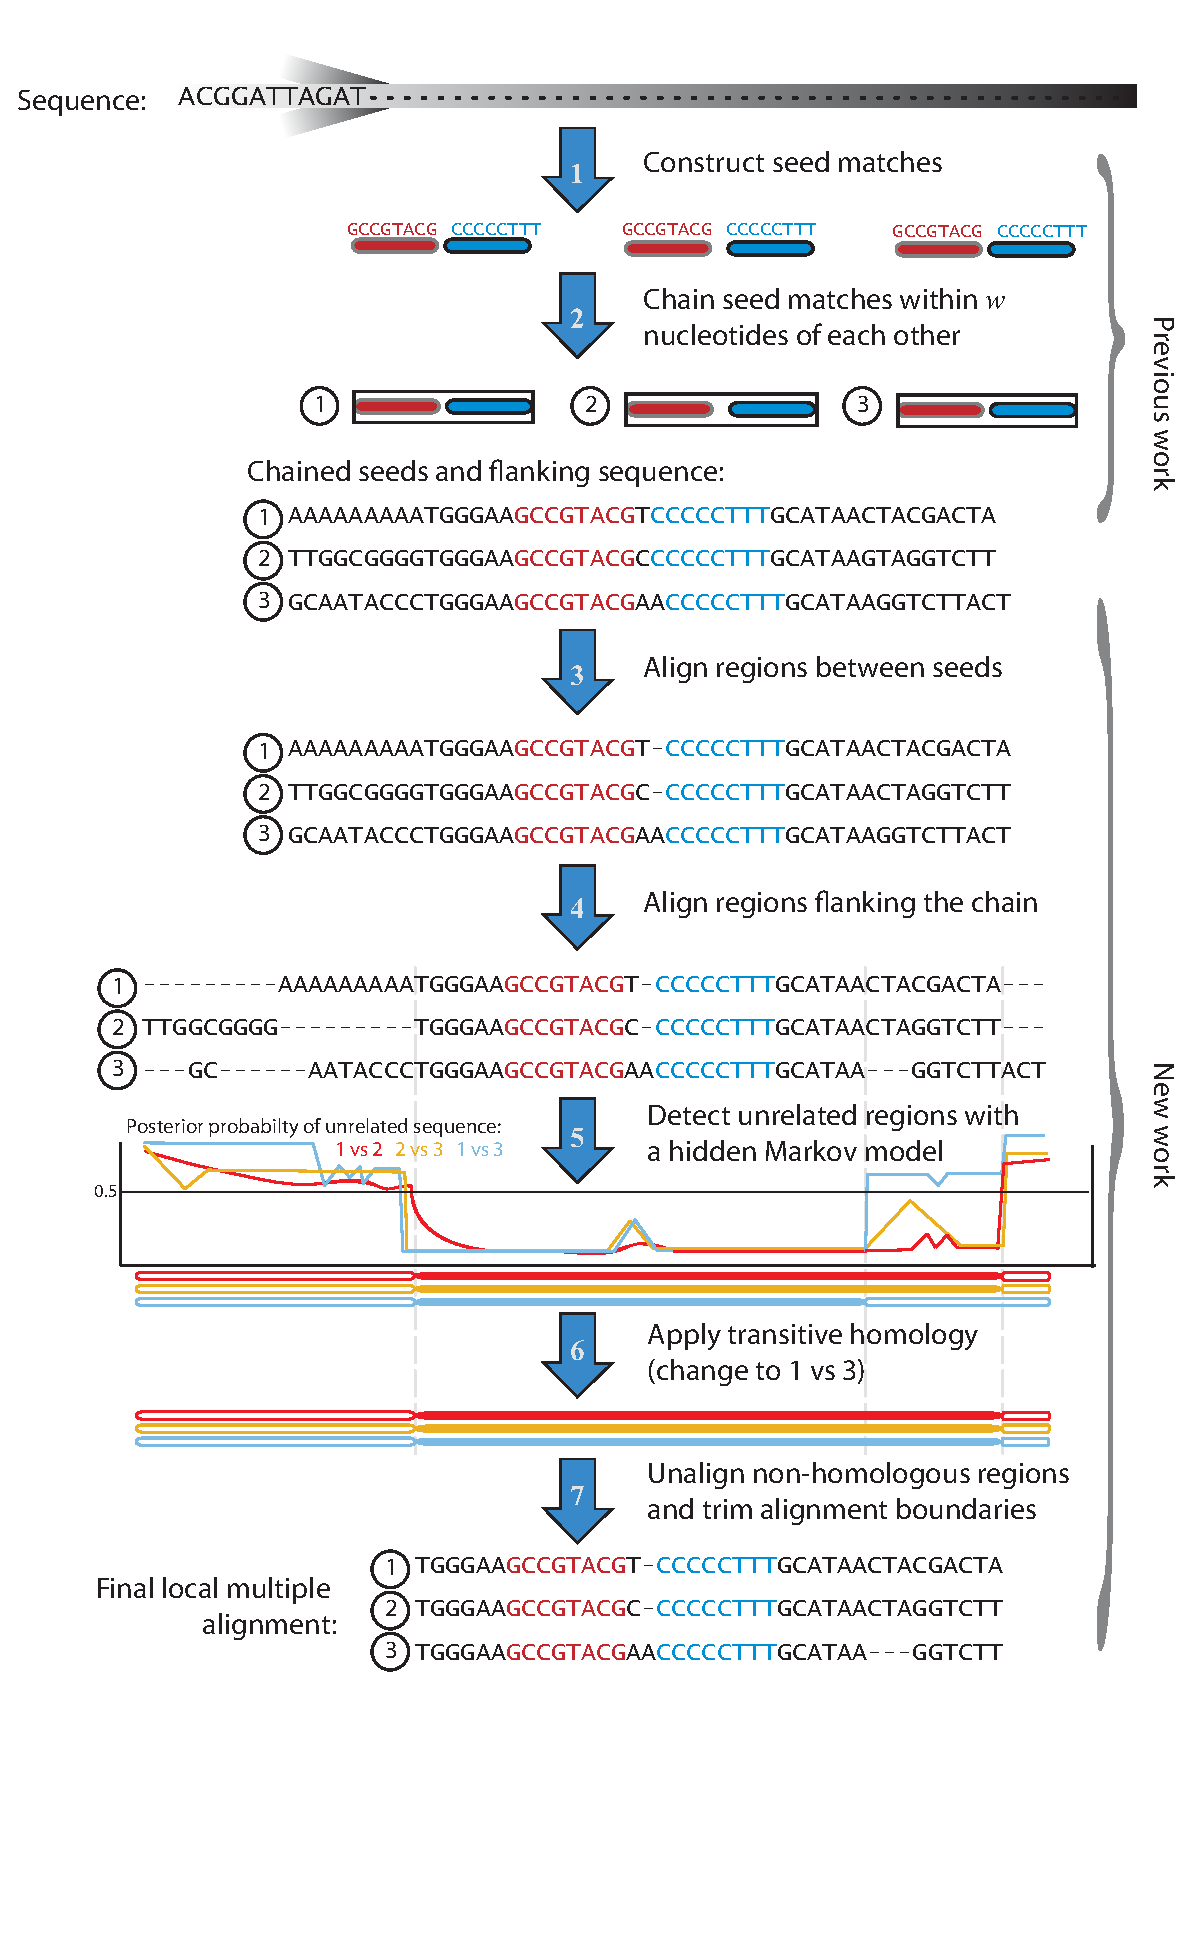
\epsfig{file=./figures/extension.eps,width=3.2in}}
\subfigure[Flowchart of the algorithmic process ]{ 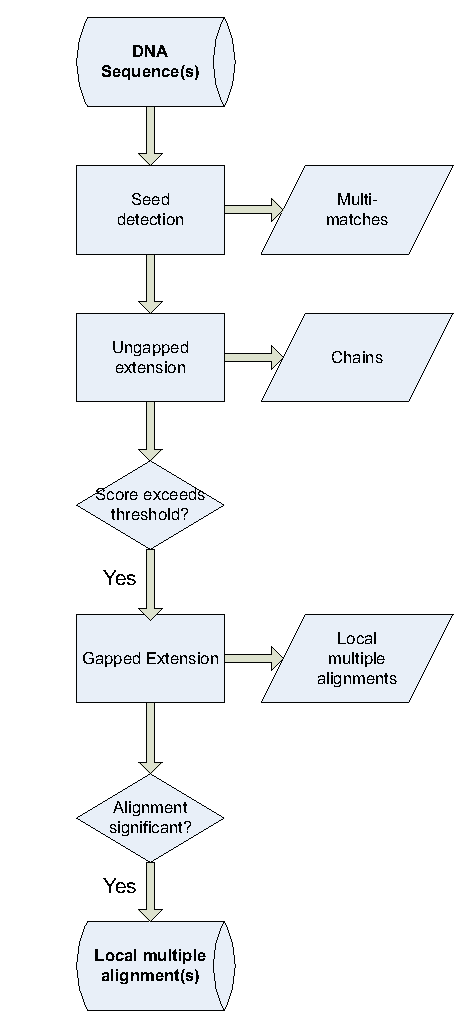
\epsfig{file=./figures/flowchart.eps,width=1.39in}}
\end{center}
\caption{Overview of the method, starting with an input sequence and ending with a set of local multiple alignments. First we (1) detect multi-matches in input sequence(s) using palindromic spaced seeds, then we perform (2) prioritized chaining of all multi-matches.  The resulting chain contains two matches and three match components labeled 1, 2, and 3.  We then perform gapped alignment of the region between chained matches (3).   In step (4), we perform a gapped extension by computing a global multiple alignment on the regions to the left and right of each chain component.  The resulting alignment may contain non-homologous sequence, so in step (5) we apply random-walk statistics to detect poorly aligned regions indicative of unrelated sequence.  In step (5), heavily diverged homologous sequences may be incorrectly classified as nonhomologous.  Step (6) computes transitive homology relationships to ensure a consistent alignment and aid detection of divergent homologous sequences.  Finally, in step (7) we unalign regions found to be non-homologous.  If we find after step (7) that the alignment boundaries have been extended, we acquire additional flanking sequence and return to step (4) for another round of extension.}
\end{figure}


%\colorbox[named]{Gray}{adfa}

\subsection{Detecting seed multi-matches}

As a starting point for homology detection, we locate all spaced seeds of a given weight $z$ in the input sequence(s). The palindromic spaced seed pattern is analyzed at each position in the input sequence to identify all multi-matches.  Previously we have demonstrated that palindromic spaced seeds offer good efficiency and sensitivity on a variety of input sequences~\cite{ref-procrast}.

\subsection{Creating chains of multi-matches}

Once we have generated a list of multi-matches, we rely on our previously described method for efficiently filtration method for chaining ~\cite{ref-procrast}. A brief review of the method follows(for additional details refer to the manuscript).

In order to chain over each region of sequence $\mathcal{O}(1)$ times,
our method chains matches in order of decreasing multiplicity--we
extend the highest multiplicity matches first. When a match can no
longer be chained without including a gap larger than $w$
characters, our method identifies the neighboring \textit{subset}
matches within $w$ characters, i.e. the light gray seed in
Figure~\ref{fig:simple_extension}. We then \textit{link} each
neighboring subset match to the chained match. We refer to the
chained match as a \textit{superset} match. Rather than immediately
extend the subset match(es), we \textit{procrastinate} and extend
the subset match later when it has the highest multiplicity of any
match waiting to be extended. When chaining a match with a linked
superset (light gray in Figure~\ref{fig:simple_extension}), we
immediately include the entire region covered by the linked superset
match--obviating the need to re-examine sequence already covered by
a previous match extension.

Once we have finished the chaining process, we would like to score and evaluate the chained multi-matches to make a decision whether its worth spending computational resources on gapped extension. This idea has been used in other local multiple alignment heuristics~\cite{...} in order to minimize the number of gapped extensions that do not improve the boundaries of the chain.

\subsection{Gapped extension of high scoring chains}

Now that we have decided to performed a gapped extension in the current direction, we use MUSCLE to align the left/right region immediately surrounding the chains. The size of the extension window we send to MUSCLE is the lesser of 4*w or 200 nucleotides. The reasoning by setting our minimum extension window to 200nt is closely related to how we determine homology borders. Since we will assume that the extension window we have decided to align with MUSCLE is homologous over its entire length, we use random walk statistics to correct our assumption.

\subsection{Identifying non-homologous regions}

The MUSCLE alignment software dutifully reports the highest scoring global multiple alignment of input sequences, regardless of whether they are homologous.  When MUSCLE aligns partially or wholly unrelated sequences, the alignment scores in the unrelated region take on negative values, as dictated by the HOXD scoring matrix and associated substitution and gap open penalties.  Random-walk statistics require a cumulative score function that trends toward negative values, but seeded alignments are expected to have large positive scores on average.  Thus, we simply invert the scoring scheme so it assigns negative values to matches and positive values for substitutions and gaps to arrive at a score with a negative expected value for seeded alignments.

When applying random walk statistics, we consider each pair of aligned sequences separately.  Given the scoring scheme, the cumulative sum of scores can be calculated for each pair of aligned nucleotides:

\begin{equation}
\label{eqn:scoresum}
S_n^\theta(a) = \sum_{i=1}^{n} Score_\theta(a_i) = S_{n-1}^\theta(a) + Score_\theta(n), S_0^\theta = 0
\end{equation}

Since the expected value $E(\theta) < 0$, partial score sums generate transient random walks.  Random stopping times can be defined recursively as:
\begin{equation}
\label{eqn:stoppingtimes}
\tau_0 = 0, \tau_1 = \min_i(S_i < S_0),\dots,\tau_{k+1} = \min_i(S_i < S_{\tau_k})
\end{equation}
where $S_n$ is defined as in Eqn.~\ref{eqn:scoresum}.  The random stopping times defined by $\tau$ form a strictly decreasing set of ladder points.  The horizontal distances (in alignment columns) between consecutive ladder points $\tau_{k+1}-\tau_{k}$ are referred to as ladder epochs.

We refer to the maximum score achieved during the $k^{th}$ ladder epoch as the Local Record Height for that epoch, as defined by:
\begin{equation}
\mathrm{LRH}_k = \max_{\tau_{k-1}\leq t \leq \tau_k}(S_t - S_{t_{k-1}})
\end{equation}
FIXME: one of the previous should be arg\{max/min\} instead of \{max/min\}.  Note that $\mathrm{LRH}_k \geq 0$.  The number of ladder epochs in an alignment with $N$ columns is denoted as $\wedge(N)$.  The distribution of the maximum value in a sequence of local record heights generated on an alignment can be approximated by an Extreme Value Distribution (EVD) parameterized as:
\begin{equation}
\label{eqn:evd}
Pr(\max_{j \leq \wedge(N)}(\mathrm{LRH}_j > x)) = \exp(-NKe^{-\mu x})
\end{equation}
Here $\mu$ is the positive solution of an equation involving the moment generating function that accounts for sequence composition and indel frequency:
\begin{equation}
mgf_\theta(\mu) = \sum_j \pi_j e^{\mu \theta\{j\}}
\end{equation}
For the HOXD substitution matrix and associated affine gap penalties this equation takes the form $mgf_\theta(\mu) = \pi_{A\leftrightarrow A}e^{91\mu} + \pi_{C\leftrightarrow C}e^{100\mu} + \pi_{G\leftrightarrow G}e^{100\mu} + \pi_{T\leftrightarrow T}e^{91\mu} + \pi_{A\leftrightarrow C}e^{-114\mu} + \pi_{A\leftrightarrow G}e^{-31\mu} + \pi_{A\leftrightarrow C}e^{-123\mu} + \pi_{C\leftrightarrow G}e^{-125\mu} + \pi_{C\leftrightarrow T}e^{-31\mu} +  \pi_{G\leftrightarrow T}e^{-114\mu} + \pi_{gapopen}e^{-400\mu} + \pi_{gapext}e^{-35\mu}$; where $\pi_j$ is the observed frequency of a column of type $j$ in the alignment.  FIXME: is this right and does it work correctly for gaps?

We estimate the values of $K$ and $\wedge(N)$ from Equation~\ref{eqn:evd} by recording the maximum LRH values observed in each each of 10,000 simulations and then fitting the functional form of Equation~\ref{eqn:evd} to the resulting distribution of extreme values.  FIXME: need to incorporate Guillaume's GC content approximation here?

Solving for $\mu$ and subsequent application of Equation~\ref{eqn:evd} enables us to deduce an approximate scoring threshold beyond which the ladder epoch in question contains non-homologous sequence with probability greater than a chosen value. 

Although we can be nearly certain that ladder epochs with a LRH exceeding our significance threshold contain an alignment of non-homologous sequence, the exact columns where the transitions between homology and non-homology take place remain ambiguous.  To determine tight boundaries on the non-homologous region, we compute ladder points for the significant region in the forward and reverse direction and call the entire region between ladder points non-homologous.

The result of applying the random-walk statistics is a prediction of non-homologous segments among each pair of aligned sequences.  The remaining regions are predicted as homologous.  We apply transitivity to these homology predictions, resulting in a final set of consistent homology predictions.  See Figure~\ref{fig:example}, steps 5 and 6 for an example. Regions found to be non-homologous are unaligned from each other.


\textbf{FIXME}: we can exceed the threshold and still improve boundaries.  If have reached the end of the extension window without going beyond our homology threshold, we then improve our original seed boundaries and then trigger another round of chaining(and consequently another round of extension) in the same direction on the currently active, extend match. Else, if we surpass the homology threshold we first determine if our chain boundaries have been improved, and then signal that we are done chaining/extending the current match in the current direction. If we have already processed the current chain in both directions, we stop entirely and proceed to the next multi-match in the priority queue.

\subsubsection{Processing Novel homologous sequence}
Its worth mentioning that novel homologous sequence can be found during gapped extension.
FIXME: should briefly describe what we do with this!


Ideally, once our algorithm finishes we will have a complete listing of all homologous local mulitple alignments. This list could be potentially overwhelming, and even at this point, we still need a way of selecting only the highly significant alignments.


\section{Results}
We have created a program called \texttt{procrastAligner} for Linux,
Windows, and Mac OS X that implements the described algorithm. Our
open-source implementation is available as C++ source code licensed
under the GPL.

\begin{figure}[t]
\scriptsize
\begin{verbatim}
GGGAGGATTGCTTGAACCTG--------GAGATTCAAGTGAGCTGAGATTGCACCACTGCATTCCAGCCTGGGC--AACAAAGCAAGACTCT-
AGGAGAATTGCTTGAACCTGGGAG-GCGGAGGTTGCAGTGAGCCGAGATGACGCCACTGCACTCCAGCCTGGGC--GACAGAGCA--------
AGGAGAATCGCTTGAACCCAAGAGAGTGAAGGTTGCAGTGAGCTGAGATCATGCCACTTCACTCCAGCCTGAGTGAAACAGC-----------
AGGAGAATAACTTCAACCTGGGAG-ACAGAGGTTGCAGTCAGCTGAGATCGCACCACTGCATTCCAGCCTGGGT--GACAGACCGAGACTCTG
AGGAGAACTGCTTGAACTCGGGAG-GCAGAGATTGCAGTGAGCTGAGATCATGTCAATGCACTGCAGCTTGAGT--GACAGAGTG--------
AGGAGAATCGCTTGAACCTGGGAG-GCAGAGGTTACAGAGAGCTGGGATTGTGCCACTGCACTCCGGCCTGGGC--AACAGAATG--------
A-CAGAATCACTTGAACCTGGGAG-GCAGAGGTTACAGTGAGCCAAAATCGCGCCACTGCACTCCAACCTGGGC--AACACAGCAA-------
AGGAGAATTGCTTGAACCCGGGAG-GTGGAGGCTGCAGTGAGCCGAGATCATGCCACTGCACTCCAGCCT-GGT--GACAGAGCGAGA-----
AGGAGAATTGTTTGAACCCAGGAG-GCGGAGGCTGCAGTGAGCCGAGATTGTGTCACTGTACTCCAGCCTGGGCAAGACAGAG----------
AGGAGAATCCCTTCAACCTGGGAA-ACAGAGGTTGCAGTGAGCCAAGATCGCACCATTGCACTCCAGTCTGGGC--AACAGAGAGA-------
*  ** *    ** ***           ***  *   * ****    **     **  * * * *    *  *      *

\end{verbatim}
\vspace{-0.5cm}
\normalsize
\caption{Partial alignment of Alu-Sc subfamily found in \emph{H. sapiens} C1 esterase inhibitor gene. Each row represents an aligned ALU.}.
\end{figure}

\subsection{Comparison with RepeatScount}

RepeatScout generates a repeat family consensus for all high frequency kmers via ungapped extension. As output, RepeatScout returns all families atleast 50nt long and occuring atleast 3 times in the input sequence(s). Once finished, RepeatScout uses RepeatMasker to locate all occurences of the repeat family in the input sequence(s).

How can we compare this to procrastAligner?


\section{Discussion}
\subsubsection{Comparison of gapped
extension approaches}


\begin{itemize}

\item RepeatScout extends one nucleotide at a time
\item ABA merges pairwise matches and resolves inconsistencies by
whorl and bulge removal
\item multiz? and HomologMiner? also merge pairwise matches, how do
they resolve inconsistency?
\item procrastAligner generates multiple alignments using libMUSCLE,
which does progressive multiple alignment.  Progressive means that
pairwise alignments do enter in at some stage, but for higher
multiplicity matches, much of the alignment is multiple alignment.
cite a paper which shows multiple alignment is more accurate than
pairwise alignment.  MUSCLE's iterative refinement procedure ensures
a high-scoring alignment irrespective of guide tree.

\end{itemize}


\subsection{Significance estimation and simulations}

Finally, we would like to extend blast statistics to multiple local alignment. How?
\begin{itemize}
\item Extending Repseek simulations to multiple
\item Tompa et al, estimating the parameters for multiple alignments
\item will involve running procrastAlign with fixed parameters on sequences varying in composition and length
\item also will have to take into account multiplicity
\item FIXME: fill in more details on Monday
\end{itemize}

\section{ Acknowledgments }
AED was supported by NSF grant DBI-0630765. TJT was
supported by Spanish Ministry MECD Grant TIN2004-03382 and AGAUR
Training Grant FI-IQUC-2005.

\bibliographystyle{splncs}
\small
\bibliography{procrastination}


\end{document}
